\documentclass[paper=A4, fontsize=11pt]{article}

\usepackage{amsmath, amsfonts, amsthm}
\usepackage{sectsty}
\allsectionsfont{\centering \normalfont\scshape}

\usepackage{fancyhdr}
\pagestyle{fancyplain}
\fancyhead{}
\fancyfoot[L]{}
\fancyfoot[C]{\thepage}
\fancyfoot[R]{}
\renewcommand{\headrulewidth}{0pt}
\renewcommand{\footrulewidth}{0pt}
\setlength{\headheight}{13.6pt}

\numberwithin{equation}{section}
\numberwithin{figure}{section}
\numberwithin{table}{section}

\setlength{\parindent}{4em}
\setlength{\parskip}{1em}
\renewcommand{\baselinestretch}{1.5}

\usepackage{graphicx}
\graphicspath{{logo/}}

\usepackage{xepersian}
\sectionfont{\fontsize{15}{10}\selectfont}
\settextfont[Path=font/]{Vazir.ttf}
\setlatintextfont{Times New Roman}

\newcommand{\horrule}[1]{\rule{\linewidth}{#1}}

\title{
\normalfont\normalsize

\includegraphics[scale=0.07]{AKUT.png}
\hspace{5cm}
%\includegraphics[scale=0.1]{ceit} \\
\\
\large \textsc دانشکده مهندسی کامپیوتر و فناوری اطلاعات
\\
\vspace{0.5cm}
\Large پرسش و پاسخ بصری با استفاده از شبکه های عصبی کانولوشنی و بازگشتی عمیق
}

\author{ علی غلامی}

\date{\normalsize\today}

\begin{document}

\maketitle

\newpage
\section{مقدمه}
\par
درك انسان از محیط اطراف خود، از ابتداي کودکی شکل می گیرد. اگر از یک کودك، درباره جهانی که براي او
قابل رویت است، سوالی پرسیده شود، بلافاصله درباره ي این جهان جملاتی توصیفی با دقت بسیار بالا ارائه می
کند. انتقال این قدرت به ماشین ها از این جهات مختلفی حائز اهمیت می باشد. یکی از جهات اصلی آن، کاربرد
هاي بی شماري است که می توان از این قابلیت در امور مختلفی استفاده کرد. دوربین هاي نظارتی، خودروهاي
خودران و ... نمونه هایی از این کاربرد ها هستند. درك تصاویر به همراه درك سوالاتی که مرتبط با آن تصاویر پرسیده می شود، می تواند یکی از اساسی ترین
قابلیت هاي یک سامانه مدیریت هوشمند تصاویر، خودروي خودران و یا یک سیستم بازیابی تصویر هوشمند باشد.
براي این منظور نیاز است که ابتدا صحنه به نمایش درآمده توسط ماشین هضم گردد. بدین معنی که بدون درك
درست از آنچه در تصویر موجود است، ساخت چنین سامانه اي امکان پذیر نخواهد بود
\section{مرور سوابق پیشین}
\par

روش هایی که جهت حل مسائل پرسش و پاسخ بصري ارائه شده اند از تنوع بالایی برخوردار هستند. اگرچه، می
توان اغلب این روش ها را در راستاي حل چهار چالش مهم زیر در نظر گرفت:
\begin{enumerate}
	\item استخراج ویژگی از تصاویر
	\item استخراج ویژگی از متن و سوالات پرسیده شده
	\item ترکیب بردار هاي ویژگی مستخرج از تصویر و متن
	\item چالش تولید پاسخ متناسب با ویژگی ها ترکیب شده
\end{enumerate}
با تحول عظیمی که در سال  2012 با ارائه مدل کانولوشنی عمیق جهت استخراج ویژگی ارائه شد و نیز افزایش
قدرت پردازشی ماشین ها، توجه به سمت شبکه هاي کانولوشنی جهت استخراج ویژگی از تصاویر بیشتر شد. با
پیشرفت این مدل ها و ترکیب آنها با مدل هاي پردازش زبان طبیعی، تولید شرح بر تصاویر نیز مورد توجه قرار
گرفت. از سال 2015 تا به اکنون، یکی از جالب ترین موضوعاتی که توجه پژوهشگران را به سمت خود جلب کرده
است، موضوع پرسش و پاسخ بصري می باشد. این موضوع ارتباط تنگاتنگی با موضوع تولید شرح بر تصاویر دارد.
به همین منظور، بسیاري از تکنییک هاي رایج در بحث شرح بر تصاویر، در موضوع پرسش و پاسخ بصري نیز مورد
توجه قرار گرفته است.

\section{طرح پیشنهادی}
\par
سیستم پرسش و پاسخ بصري مطرح در این گزارش، به زبان پایتون و با استفاده از چارچوب کاري
تنسورفلو پیاده سازي خواهد شد. هسته این چارچوب کاري به زبان سی پلاس پلاس و با استفاده از پلتفرم توسعه
موازي کودا پیاده سازي شده است. این چارچوب کاري توسط تیم گوگل برین در حال توسعه بوده و پشتیبانی
می شود.
ایده ي اصلی مطرح در این چارچوب کاري، بیان محاسبات در قالب گراف است. هر گره ي این گراف، یک واحد
محاسباتی را مشخص می کند. با این رویکرد می توان شبکه هاي پیچیده را به راحتی پیاده سازي نمود.

\section{محصولات طرح}
\par
خروجی هاي این طرح شامل موارد زیر خواهند بود:
\begin{itemize}
\item بازیابی تصاویر در شبکه های اجتماعی با استفاده از جستجوی متن
\item توصیف کننده جهان اطراف جهت استفاده نا بینایان و مذاکره دو طرفه
\item ربات های امداد گر در عملیات هایی که با انسان تبادل اطلاعات انجام می دهند
\item ربات های مذاکره کننده
\end{itemize}


\newpage
\section{مراحل انجام}
\par
\begin{enumerate}
\item شناسایی و تهیه منابع:
	\begin{itemize}
			\item پیدا کردن مقالات مربوط به پرسش و پاسخ بصری
			\item یافتن توضیحات مربوط به طرح های از پیش پیاده سازی شده
	\end{itemize}

\item تنظیم ساختار:
	\begin{itemize}
			\item تهیه ي بخشهاي مقدمه، محتواي اصلی، چیکده، نتیجه گیري و منابع
			\item مشخص کردن ترتیب مباحث محتوا
			\item تهیه ي فهرست مباحث اصلی و فرعی یافتن معماری شبکه های کانولوشنی
	\end{itemize}

\item مطالعه و یادداشت برداری:
	\begin{itemize}
		\item پیدا کردن مقالات مربوط به پرسش و پاسخ بصری
		\item یافتن توضیحات مربوط به طرح های از پیش پیاده سازی شده
	\end{itemize}

\item اجرای بخش عملی:
	\begin{itemize}
			\item پیاده سازی شبکه های کانولوشنی عمیق 
			\item پیاده سازی شبکه بازگشتی عمیق
			\item آموزش شبکه 
			\item آزمایش و ارزیابی
	\end{itemize}

\item تهیه گزارش نهایی:
	\begin{itemize}
			\item مستند سازي و نوشتن گزارش نهایی
			\item آمادگی جهت ارائه ي شفاهی
	\end{itemize}
\end{enumerate}

\newpage
\section{زمان بندی پروژه}
\par
زمان بندی پروژه بر اساس ”پیشنهاد زمان بندی پروژه کارشناسی“ در کتاب انجام شده است.

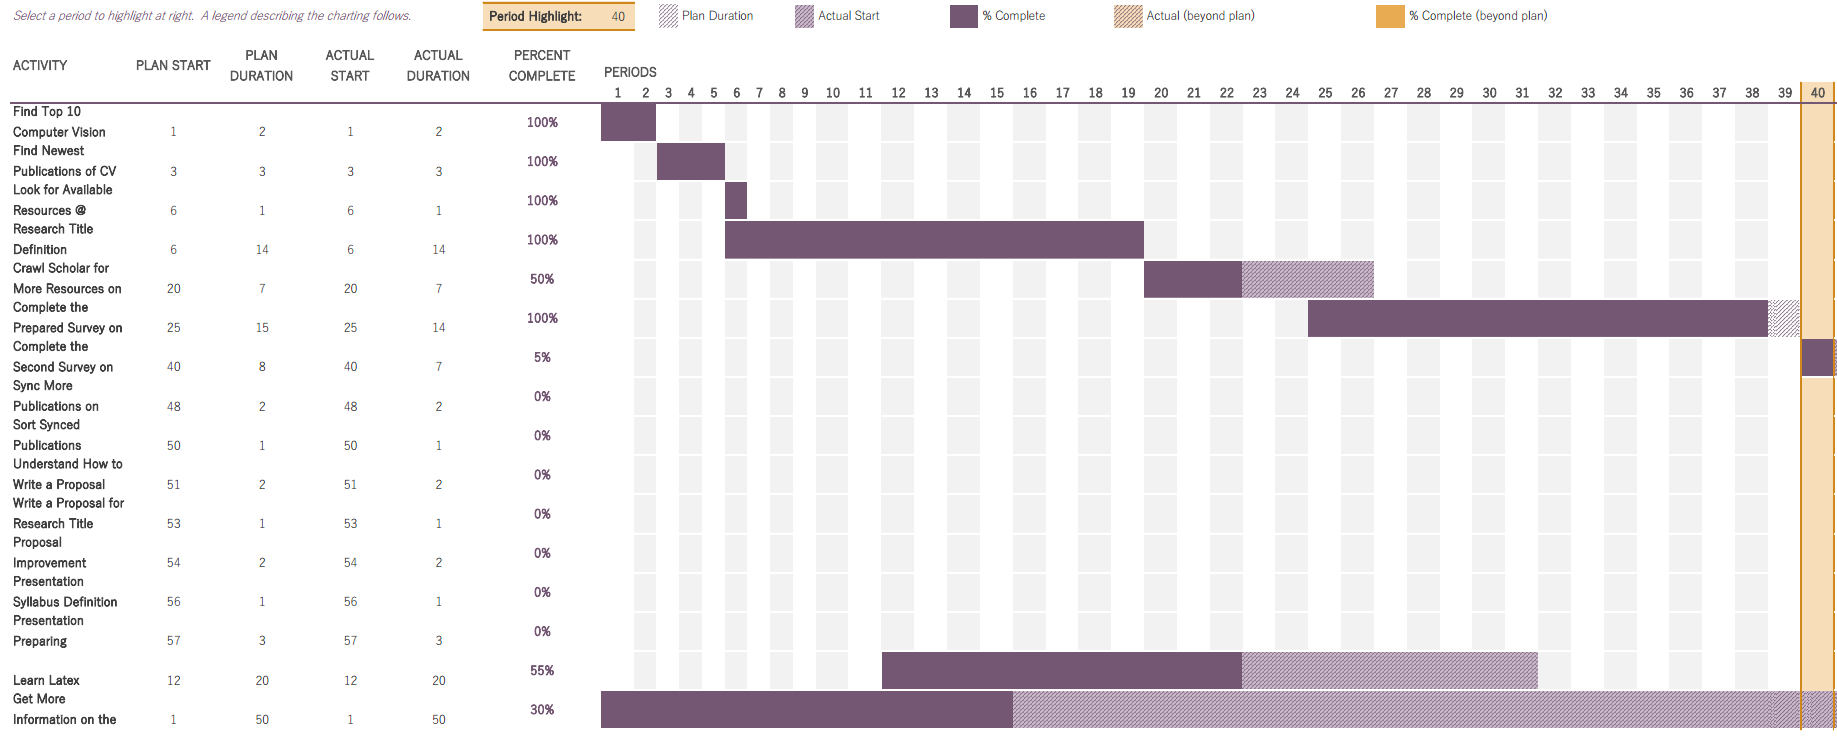
\includegraphics[scale=0.25]{gantt}
\par

\end{document}
